\section{Robotic arm Kinematic Analysis}

\begin{frame}
\frametitle{Forward Kinematics}
\begin{columns}
\column{0.2\textwidth}
\begin{figure}[htbp]
\centering
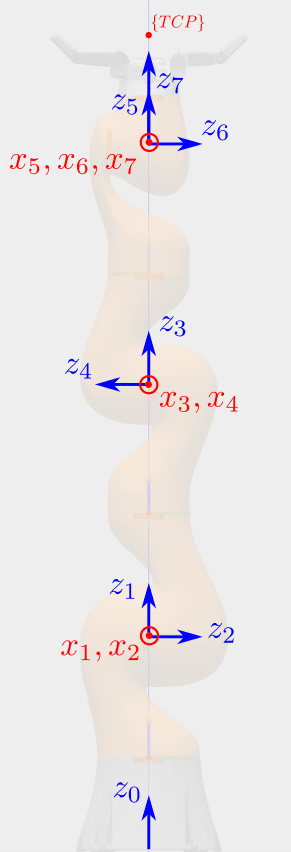
\includegraphics[width=\textwidth]{../images/iiwa-frames.png}
\end{figure}
\column{0.7\textwidth}
\begin{table}[htbp]
\begin{center}
\begin{tabular}{ |c|c|c|c|c| } 
\hline
$i$ & $θ_i$ (rad) & $L_{i-1}$ (m) & $d_i$ (m) & $α_{i-1}$ (rad) \\
\hline
1 & $θ_1$ & 0 & 0.36 & 0 \\
2 & $θ_2$ & 0 & 0 & $-π/2$ \\
3 & $θ_3$ & 0 & 0.36 & $π/2$ \\
4 & $θ_4$ & 0 & 0 & $π/2$\\
5 & $θ_5$ & 0 & 0.4 & $-π/2$ \\
6 & $θ_6$ & 0 & 0 & $-π/2$ \\
7 & $θ_7$ & 0 & 0 & $π/2$ \\
\hline
\end{tabular}
\end{center}
\caption{D-H parameters for Kuka iiwa14}
\end{table}
\[
^{i-1}T_i = 
\begin{bmatrix}
c\theta_i & -s\theta_i & 0 & L_{i-1} \\
s\theta_ica_{i-1} & c\theta_ica_{i-1} & -sa_{i-1} & -sa_{i-1}d_i \\
s\theta_isa_{i-1} & c\theta_isa_{i-1} & ca_{i-1} & ca_{i-1}d_i \\
0 & 0 & 0 & 1\\
\end{bmatrix}
\]
\end{columns}
\end{frame}

\begin{frame}
\frametitle{Inverse Kinematics - Decoupling Technique}
Solve separately for position and orientation (assume $θ_3 = 0$)
\begin{columns}
\column{0.4\textwidth}
\begin{center}
\begin{figure}[htbp]
\centering
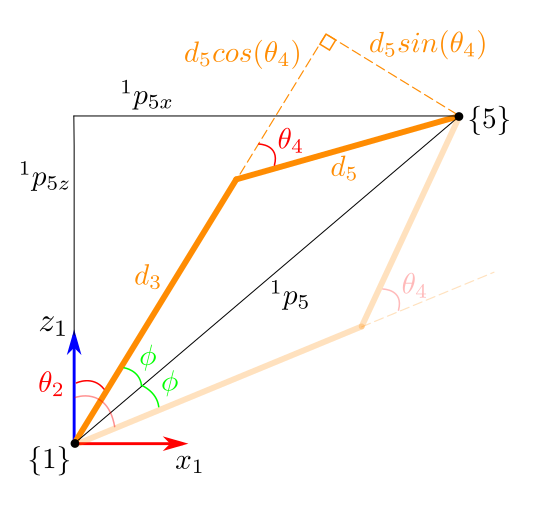
\includegraphics[width=\textwidth]{../images/th2-4-calculation.png}\\
\end{figure}
\[
{}^0\mathbf{p}_5 = {}^0T_4 {}^4\mathbf{p}_5 = \begin{bmatrix} p_x \\ p_y \\ p_z \\ \end{bmatrix}
\]
\end{center}

\column{0.6\textwidth}

\[
R_{target} = 
\begin{bmatrix}
i_x & j_x & k_x\\
i_y & j_y & k_y\\
i_z & j_z & k_z\\
\end{bmatrix}
\]
\begin{center}
\begin{figure}[!htb]
\centering
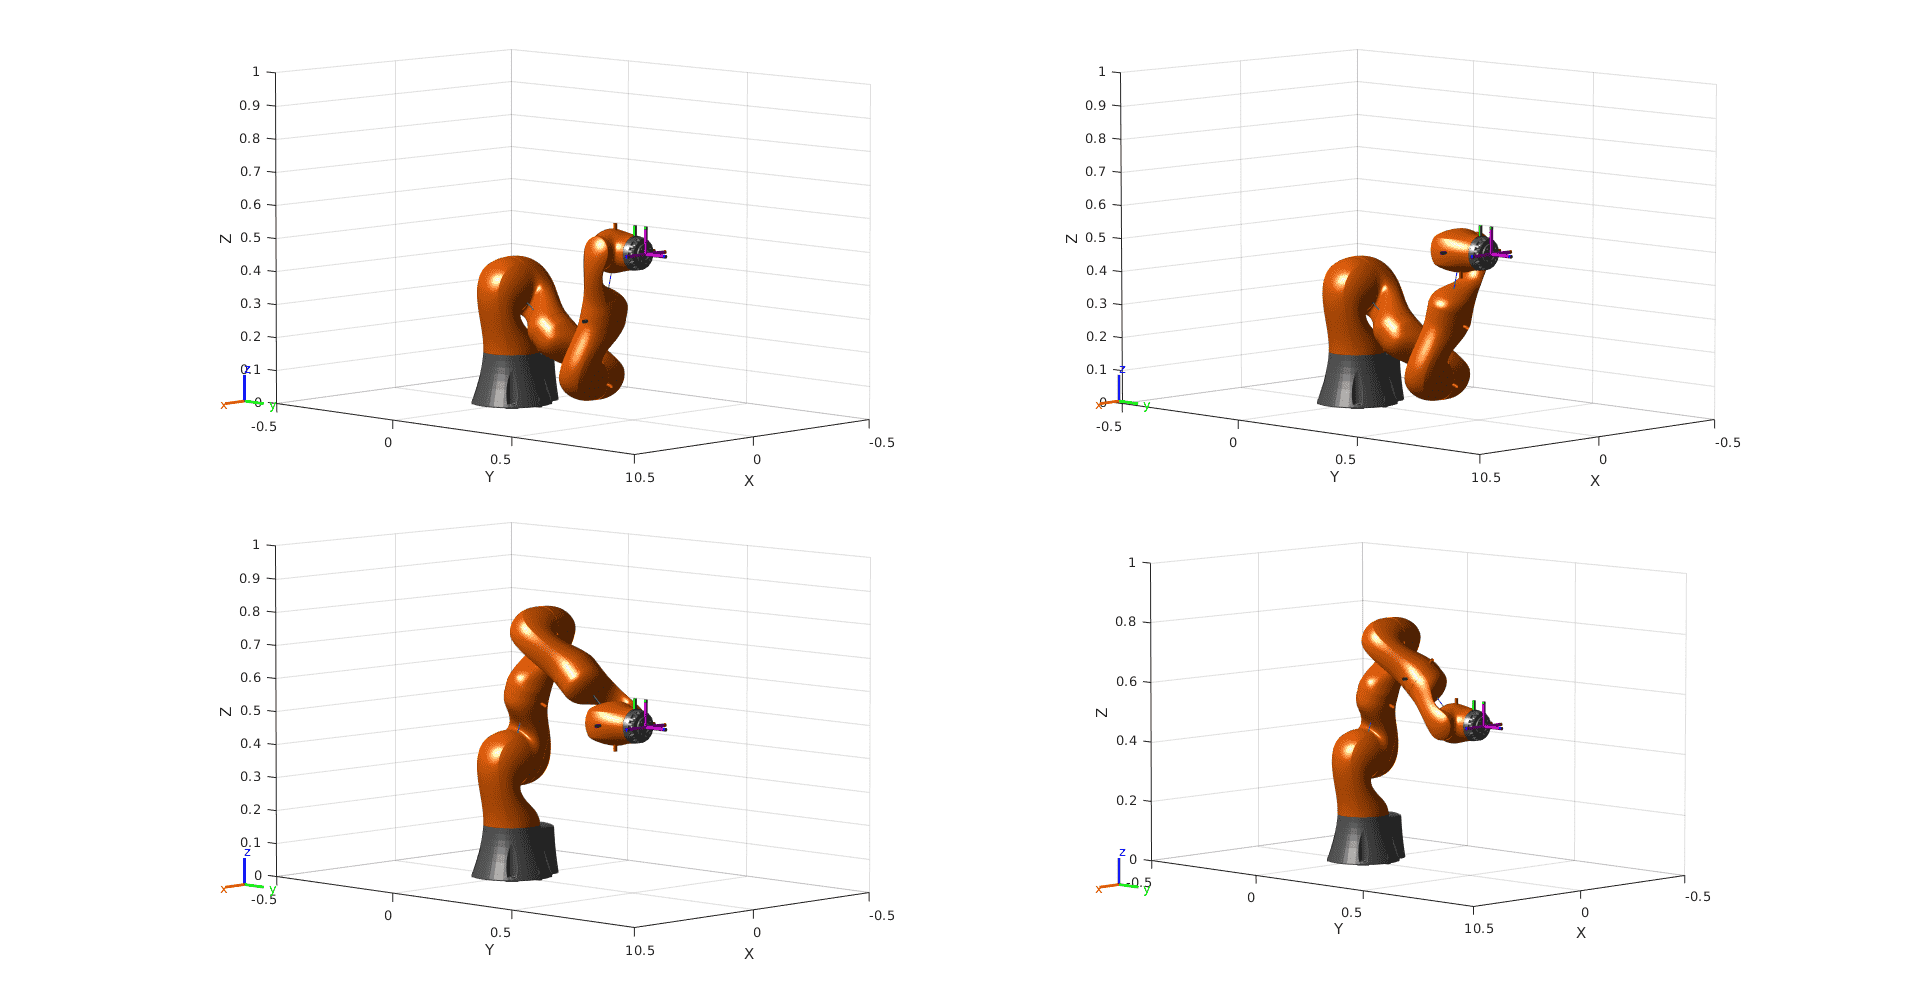
\includegraphics[width=0.9\textwidth]{../images/ik-4-solutions.png}\\
\caption{The first 4 out of 8 solutions of the IK-problem}
\end{figure}
\end{center}
\end{columns}
\end{frame}


\begin{frame}
\frametitle{Singularity points}
\begin{columns}
\column{0.8\textwidth}
\begin{itemize}
\item points where robot has \textbf{reduced kinematic capability}
	\begin{itemize}
	\item cannot move in some directions
	\item cannot move at all
	\item points where small displacements/velocities in the taskspace require very large displacements/velocities in the joint space
	\item kinematics equations are not defined or $\Vert J \Vert = 0$
	\end{itemize}
\item must be known before path planning in order \textbf{to be avoided}
\item example singularity points (based on KUKA's Sunrise.OS 1.11 manual)
	\begin{itemize}
	\item shoulder fully extended $\Rightarrow θ_1$ and $θ_3$ are not defined (there are infinite combinations for the same result)
	\item When $\sin\left( θ_6 \right) = 0$ then the angles $θ_5, θ_7$ are not defined. (infinite number of combinations of
	$θ_5, θ_7$ to get the same orientation on the end-effector.
	\end{itemize}
\end{itemize}
\column{0.2\textwidth}
\begin{figure}[htbp]
\centering
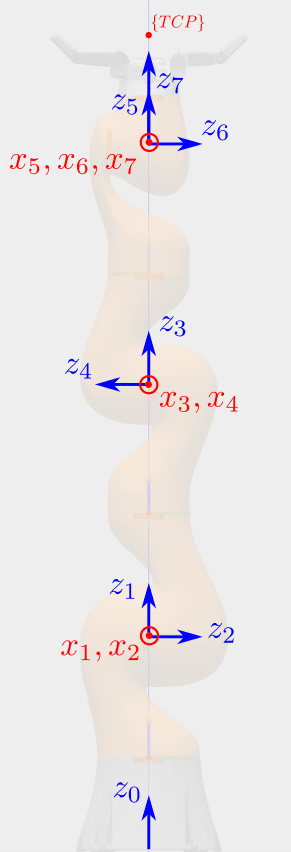
\includegraphics[width=\textwidth]{../images/iiwa-frames.png}
\end{figure}
\end{columns}
\end{frame}


\begin{frame}
\frametitle{RCM constraint}
\begin{center}
\begin{figure}[H]
\centering
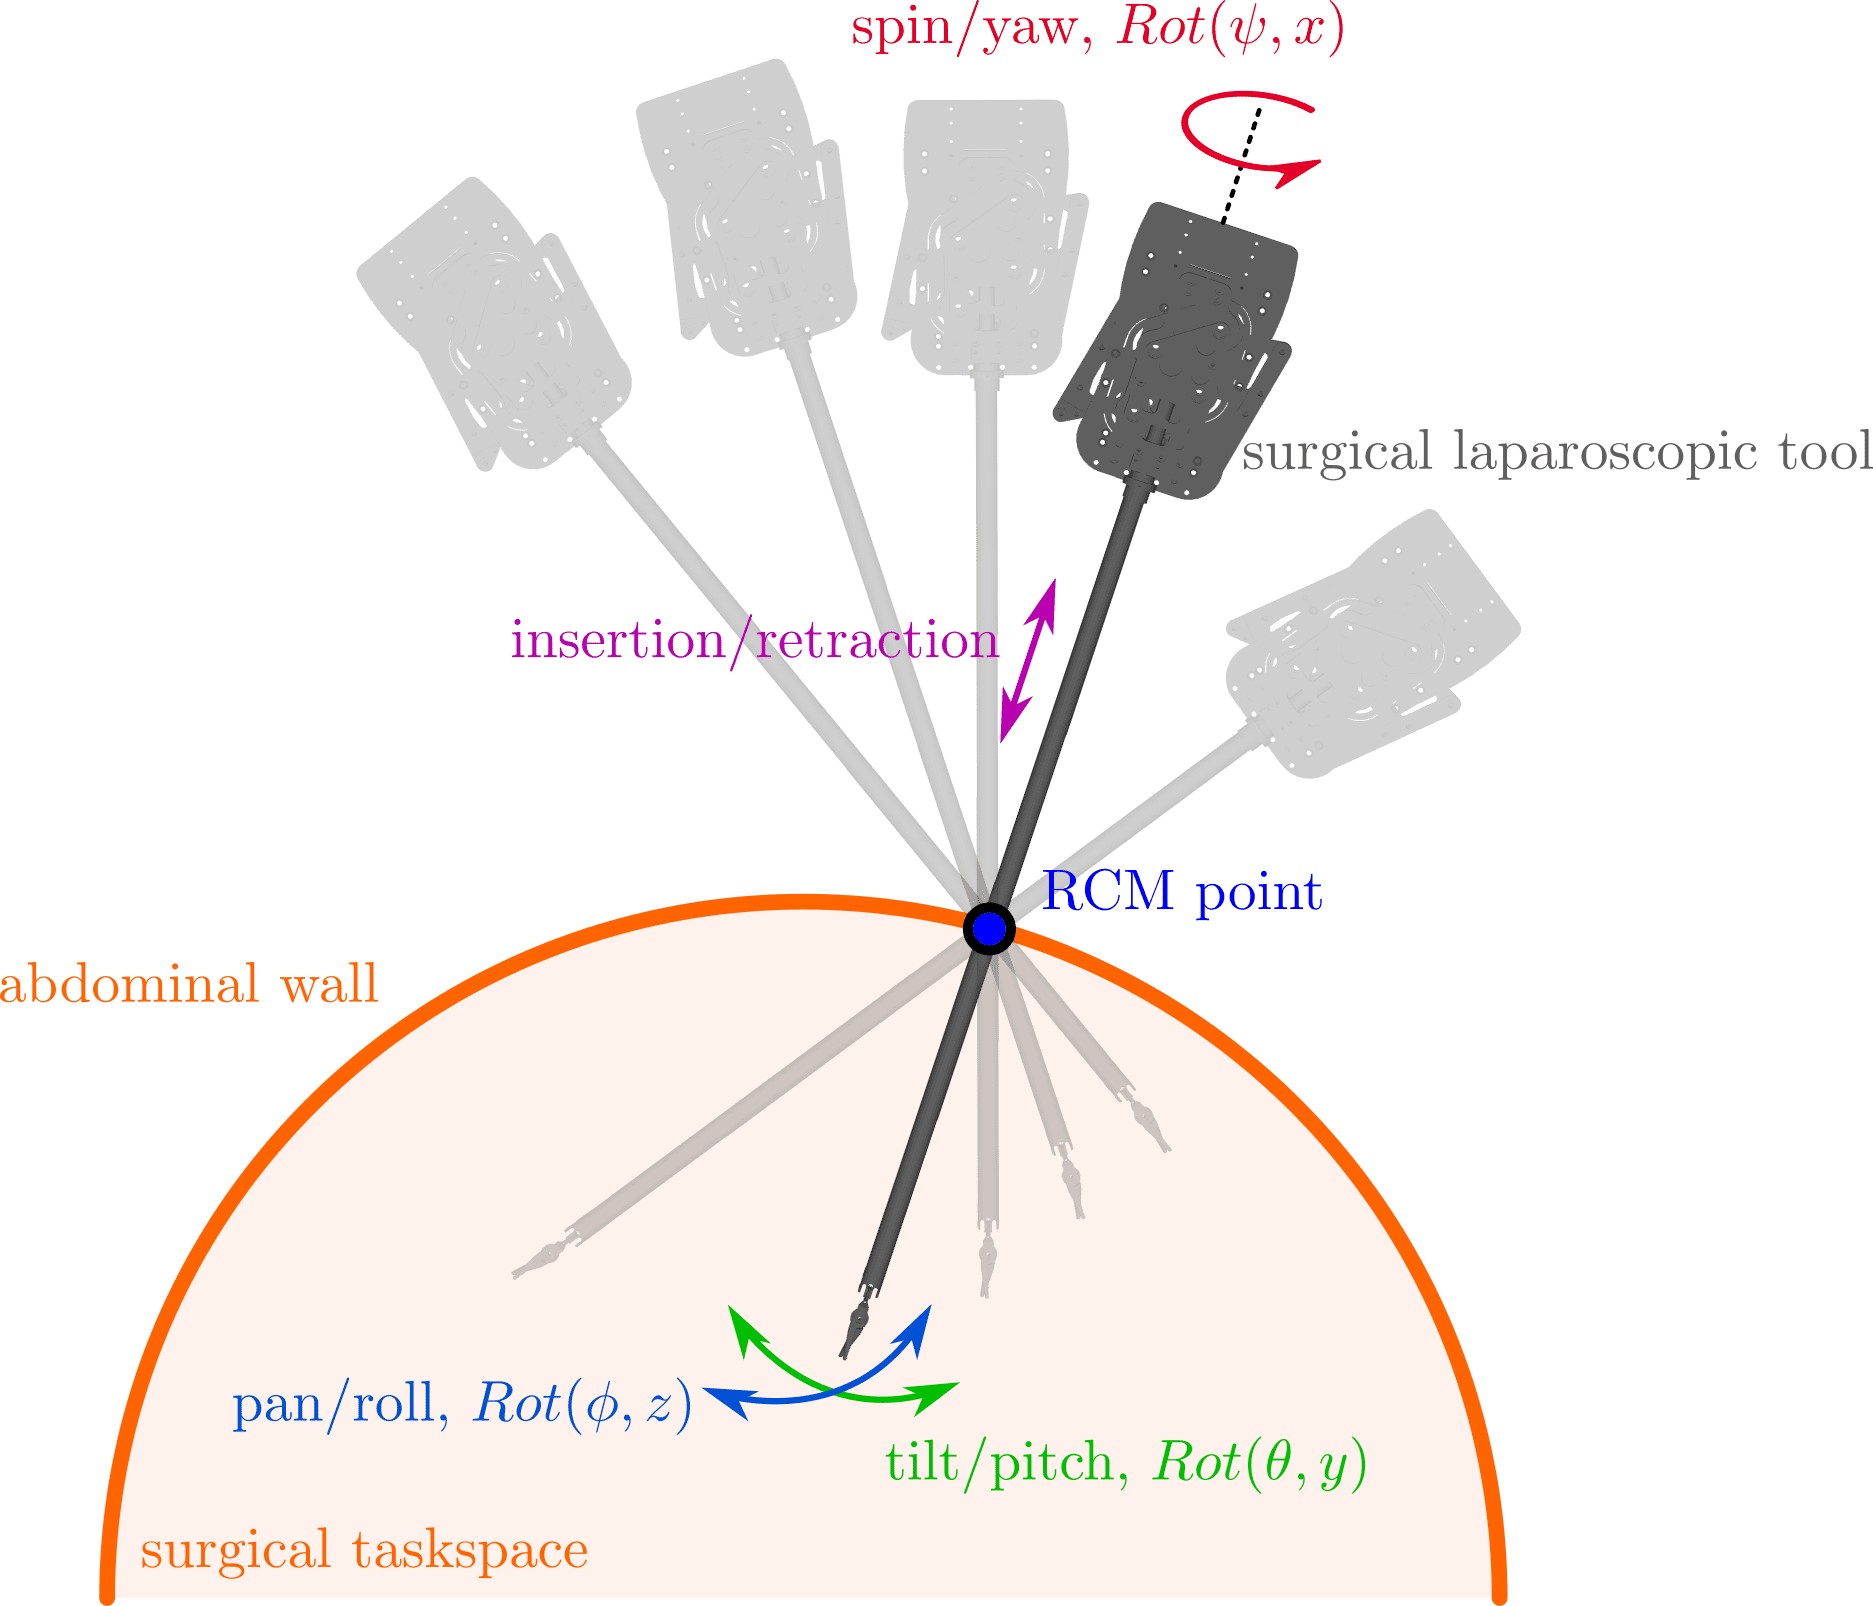
\includegraphics[width=0.5\textwidth]{../images/rcm-surgical-tool.png}\\
\caption{Illustration of pivoting motion of surgical laparoscopic tool around RCM point (also known as fulcrum or trocar point). Due to the RCM constraint, the tool has only 4 degrees of freedom.}
\end{figure}
\end{center}
\end{frame}

\begin{frame}
\frametitle{Elbow-up constraint}
\begin{columns}
\column{0.4\textwidth}
\begin{figure}[htbp]
\centering
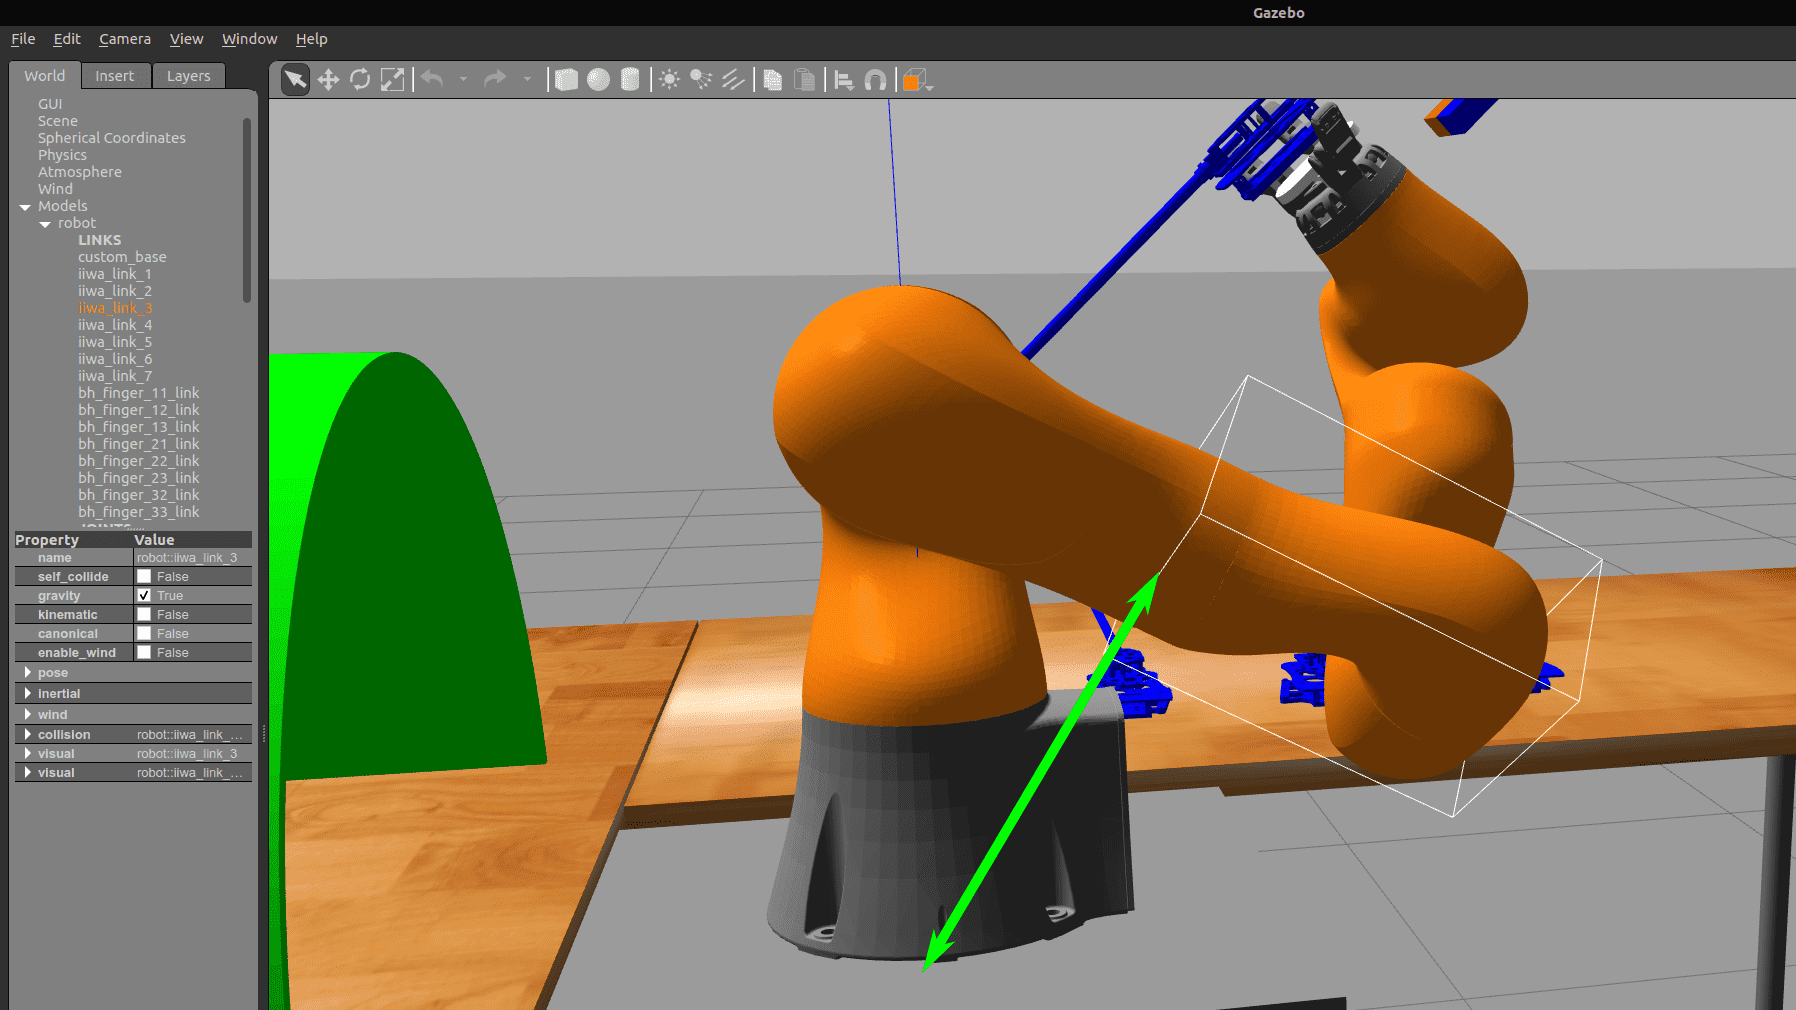
\includegraphics[width=\textwidth]{../images/elbow-down.png}\\
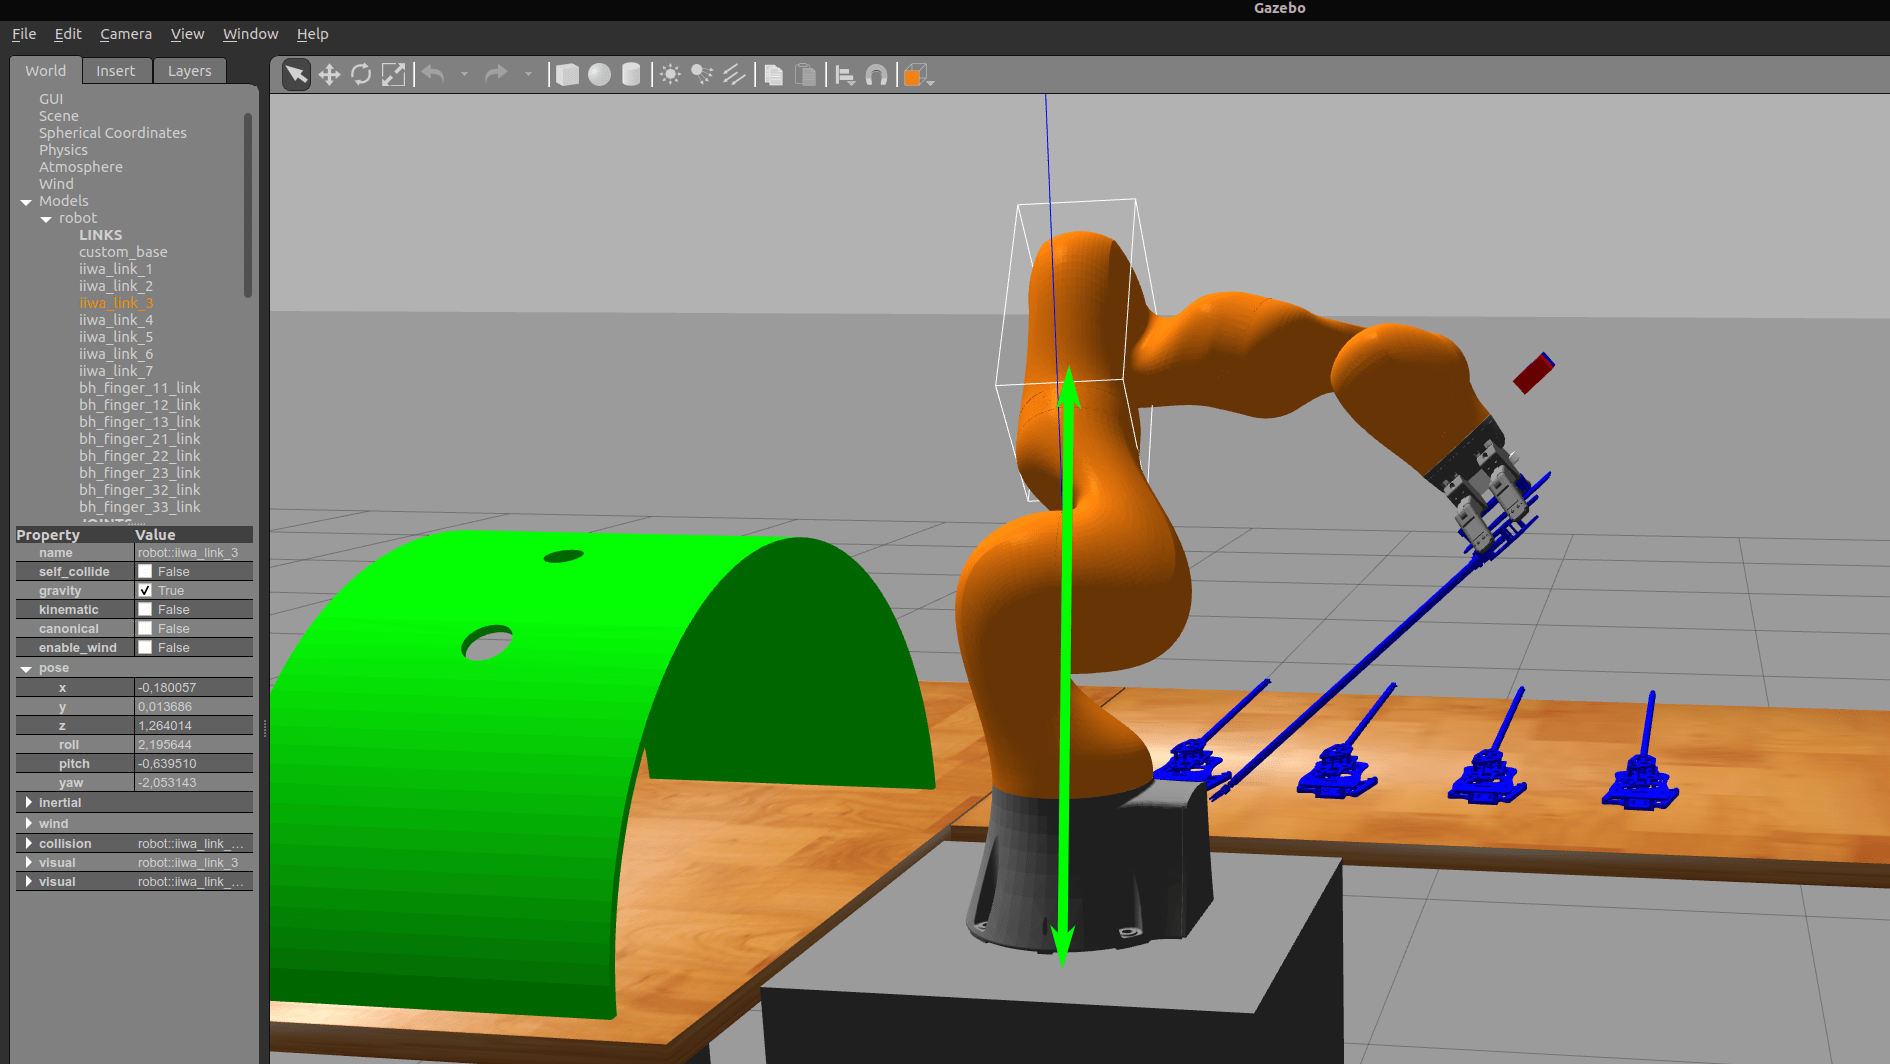
\includegraphics[width=\textwidth]{../images/elbow-up.png}\\
\caption{Top: elbow-down solution, bottom: elbow-up solution}
\label{elbow-up-vs-down}
\end{figure}

\column{0.6\textwidth}
\begin{figure}[htbp]
\centering
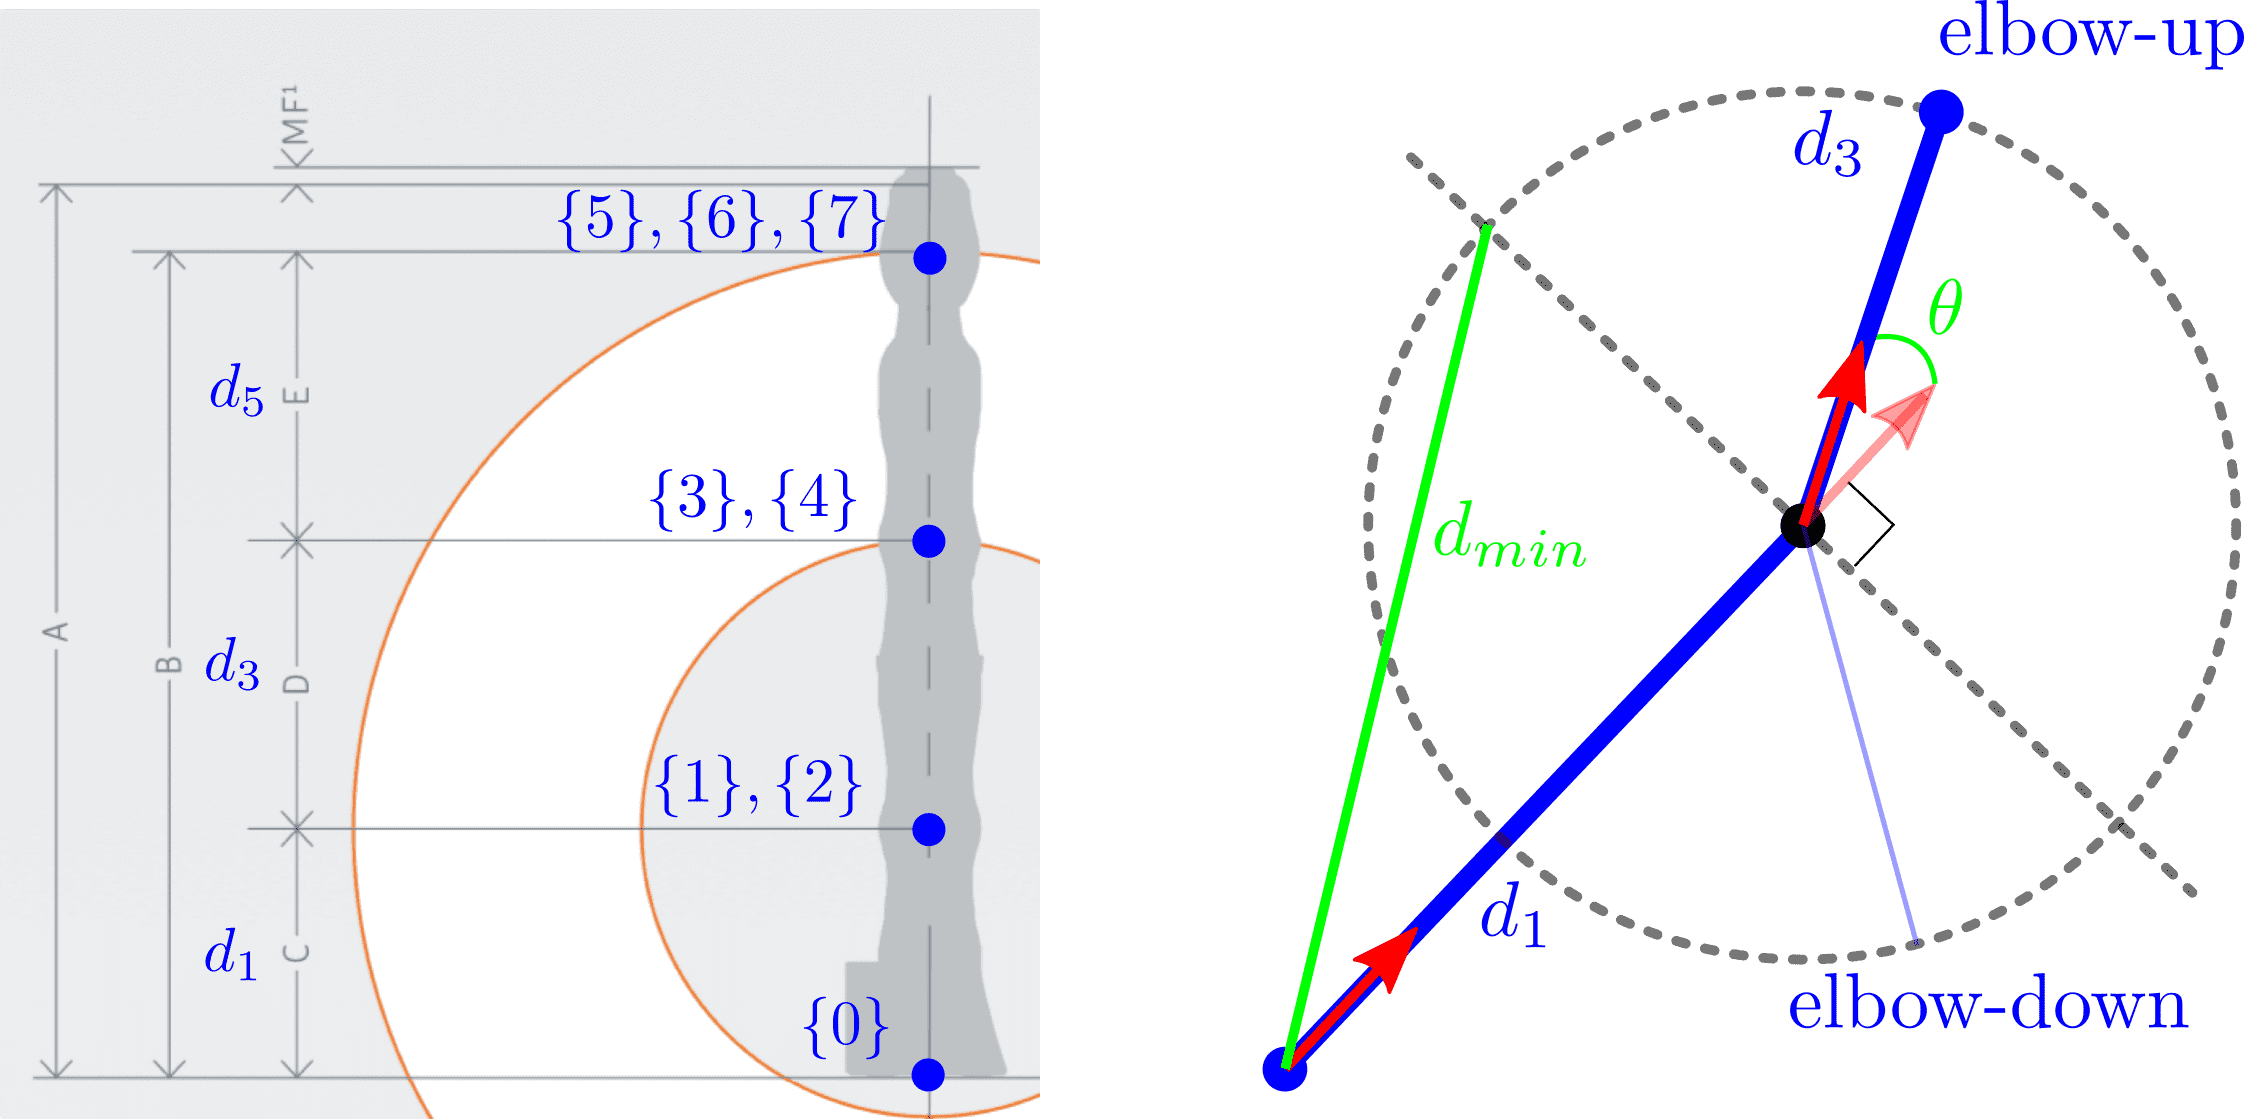
\includegraphics[width=0.8\textwidth]{../images/elbow-up-constraint-geometry.png}\\
\caption{Elbow-up constraint description with relative distance or angle between links with lengths $d_1$ and $d_3$}
\label{elbow-up-constraint-geometry}
\end{figure}

\begin{center}
$d_{\min} \leq d \leq d_{\max}$,
where
$d_{\min} = \sqrt{d_1^2 + d_3^2} = 553$mm and $d_{\max} = d_1 + d_3 = 780\mbox{mm}.$
\end{center}
\end{columns}
\end{frame}
